\documentclass[10pt,a4paper]{article}
\usepackage{amssymb} %mathbb
\usepackage{amsmath} %align
\usepackage{graphicx} %jpg
\usepackage{cancel}
\usepackage{hyperref} %a href
\usepackage{gensymb}
\usepackage{colortbl}
\usepackage{amsthm}
\newtheorem{exercise}{Exercise}
\newtheorem{definition}{Definition}
\newtheorem{thm}{Theorem}
\newtheorem{example}{Example}
\usepackage[top=1.0cm,bottom=1.3cm,left=1.0cm,right=1.0cm]{geometry}

\begin{document}

Hey, Tony Scott, my work dialogues with yours. In your Physics' language:

\begin{align}
  e^{-2xR} &= a_0 b_0 (x - r_1) (x - r_2)
\end{align}

In my language, we search for $x$ such that:

\begin{align}
  e^{xt} &= f_1(t) + x \cdot f_2(t) + \cfrac{x^2}{2} \cdot f_3(t)
\end{align}

Translating:

\begin{align}
  t &= -2R \\
  f_1(-2R) &= a_0 b_0 r_1 r_2 \\
  f_2(-2R) &= - a_0 b_0 (r_1 + r_2) \\
  f_3(-2R) &= 2 a_0 b_0
\end{align}

Consider our common case, where exponential's graph intersects parabola's graph at three real and distinct points $P_1 = (x_1, e^{x_1 t})$, $P_2 = (x_2, e^{x_2 t})$ and $P_3 = (x_3, e^{x_3 t})$.

		\begin{center}
		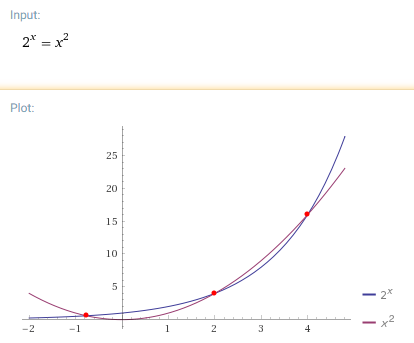
\includegraphics{2xx2}
		\end{center}

I discovered that we are, as a matter of fact, working with a cubic polynomial:

\begin{align}
\left(\begin{matrix}\exp{x_1 t} \\ \exp{x_2 t} \\ \exp{x_3 t} \end{matrix}\right) &= \left(\begin{matrix}1 & x_1 & {x_1^2}/{2}  \\ 1 & x_2 & {x_2^2}/{2} \\ 1 & x_3 & {x_3^2}/{2} \end{matrix}\right) \cdot \left(\begin{matrix}f_1(t) \\ f_2(t) \\ f_3(t) \end{matrix}\right) \\
E &= T F \\
\exp M \cdot T^\top &= \left(\begin{matrix}\exp{x_1 t} & \exp{x_2 t} & \exp{x_3 t} \\ e_1' & e_2' & e_3'  \\ e_1'' & e_2'' & e_3'' \end{matrix}\right) \\
M &= \left(\begin{matrix}0 & 1 & 0  \\ 0 & 0 & 1 \\ P & -S_2 & S_1 \end{matrix}\right) \\
x^3 - S_1 x^2 + S_2 x - P &= 0 = (x - x_1)(x - x_2)(x - x_3) \\
S_1 &= x_1 + x_2 + x_3 \\
S_2 &= x_1 x_2 + x_1 x_3 + x_2 x_3 \\
P &= x_1 x_2 x_3
\end{align}

Our common Ordinary Differential Equation is $y'''(t) - S_1 y''(t) + S_2 y'(t) - P y(t) = 0$.

\vspace{3mm}

It's a bright June afternoon and we want, at least, to isolate $S_1, S_2$ and $P$. Vinicius Claudino Ferraz, 3/Jun/2019

\end{document}
